\subsection{问题分析与联合资源模型}

问题三包含三个相互衔接的任务：在总算力约束下联合配置模型规模、训练数据量、领域配比和数据治理质量；比较不同质量成本与上下文长度对配置结果的影响；识别预算变化是否引起质量状态、配方支持或资源份额的结构性转移。本文把前两问的输出固定为响应模型参数，把问题三写成一个可复算的条件优化问题。总体接口见图~\ref{fig:q3_1}。

\begin{figure}[htbp]
\centering
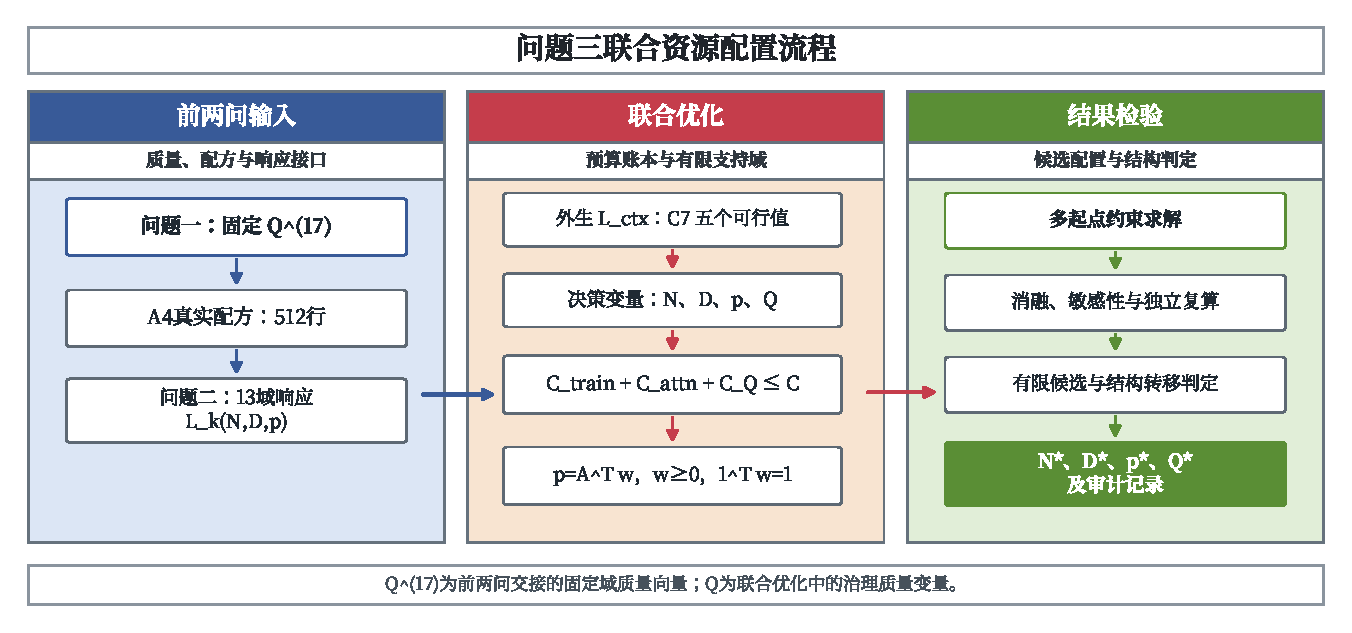
\includegraphics[width=.82\textwidth]{figures/flow_overall_model.pdf}
\caption{质量、配方及规模响应的衔接与联合求解流程}\label{fig:q3_1}
\end{figure}

\subsubsection{数据接口与变量定义}

A4 的 512 行真实训练配方给出领域配比的可行范围；第二问交付的 13 个评测域响应给出配比、规模和质量的 Loss 映射；C7 的五个上下文长度作为外生情景；B7 提供整体治理质量的条件响应。A6--A11用于复算交接响应在检验配方上的一致性，A12--A15保留为外推情景的边界参考。问题三的数值结论均指向这套已交接的响应函数。

问题一得到的 17 域质量向量记为 $\mathbf q=\mathbf Q^{(17)}$。它是固定的领域属性，其中只有 6 个不同取值；问题三另设标量 $Q$ 表示整体治理后的质量等级，并将其同时放入质量响应和治理成本。17 域治理提升不单独设变量，统一由 $Q$ 表示。定义

\begin{equation}\label{eq:q3_1}
n=\frac{N}{10^9},\qquad d=\frac{D}{10^9},\qquad
q_{\mathrm{mix}}=\sum_{i=1}^{17}p_iq_i,\qquad
Q_{\mathrm{base}}=\frac{1}{17}\sum_{i=1}^{17}q_i=0.6219326581.
\end{equation}

其中 $N$ 为参数量，$D$ 为训练 Token 数，$\mathbf p=(p_1,\ldots,p_{17})$ 为训练配方，$Q\in[Q_{\mathrm{base}},1]$ 为治理质量。训练平均配方加权基线 $0.6193580512$作为基线敏感性情景；B7 的校准点 $Q_0=0.6$只用于第二问标尺，和本问的 $Q_{\mathrm{base}}$ 分开记账。

A4覆盖三个直接观测尺度，问题三在配方方向上使用 A4 的有限凸包；$N$ 和 $D$ 的计算范围为 $[10^6,10^{11}]$ 与 $[10^9,10^{13}]$。因此，表中结果表示在交接响应下的条件配置，预算、上下文和质量成本的变化均可以由公式复算。

\begin{figure}[htbp]
\centering
\begin{subfigure}[b]{.48\textwidth}
\centering
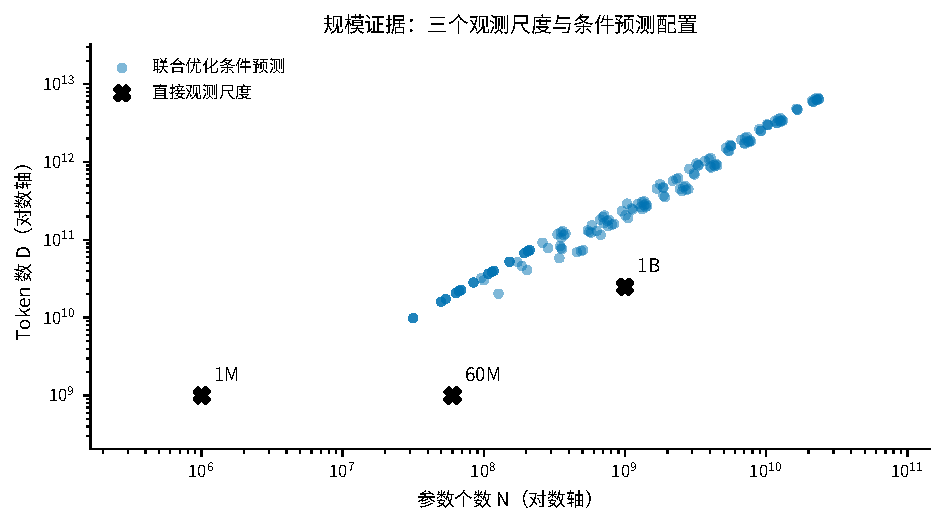
\includegraphics[width=.98\linewidth]{figures/raw_q3_scale_support.pdf}
\caption{直接支持尺度与联合配置}
\label{fig:q3_2}
\end{subfigure}\hfill
\begin{subfigure}[b]{.48\textwidth}
\centering
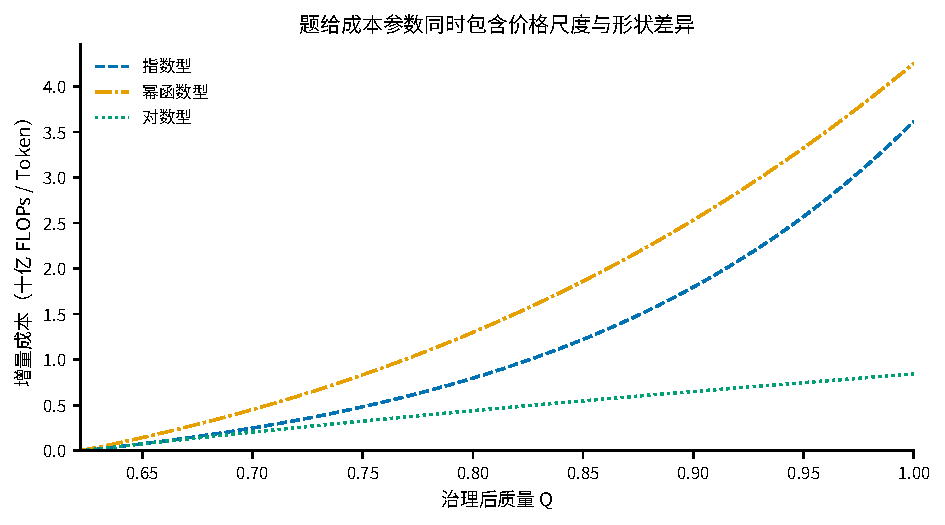
\includegraphics[width=.98\linewidth]{figures/process_q3_quality_cost.pdf}
\caption{三种质量成本的增量曲线}
\label{fig:q3_3}
\end{subfigure}
\end{figure}

\subsubsection{配方响应与质量桥接}

为适应配比的组成数据结构，对 $p_i$ 加入 $\delta=0.001$ 后作中心化对数比变换，并将质量加权配比与配方结构拼接为 34 维特征：

\begin{equation}\label{eq:q3_2}
\operatorname{clr}_{\delta}(p)_i=\ln(p_i+\delta)-\frac{1}{17}\sum_{j=1}^{17}\ln(p_j+\delta),
\qquad \delta=0.001.
\end{equation}

\begin{equation}\label{eq:q3_3}
x=(p\odot\mathbf q,\operatorname{clr}_{\delta}(p)),\qquad
z=\frac{x-\mu}{\sigma},\qquad
\Phi_k=s_k(\beta_{0k}+\boldsymbol\theta_k^{\mathsf T}z-c_k).
\end{equation}

其中 $k=1,\ldots,13$ 对应评测域，$\mu,\sigma,\beta_{0k},\boldsymbol\theta_k,s_k,c_k$ 均取第二问交接文件的全精度参数。规模项与第 $k$ 个评测域的基础响应为

\begin{equation}\label{eq:q3_4}
S_k=(n/0.001)^{-\eta_k}(d/1)^{-\zeta_k},\qquad
L_{2,k}=E_k+A_kn^{-\alpha}+B_kd^{-\beta}+S_k\Phi_k,
\end{equation}

其中 $\alpha=\beta=0.2931826439$。为把 B7 质量标尺接入 13 域响应，先写出

\begin{equation}\label{eq:q3_5}
F_7(n,d,Q)=0.9654077057+0.5307187920n^{-0.2825}
              +1.6157571765(dQ)^{-0.108}.
\end{equation}

主模型采用比值桥接，并用加性桥接做成本和桥接形式的敏感性检验：

\begin{equation}\label{eq:q3_6}
\begin{aligned}
L_k^{(r)}&=L_{2,k}\left[\frac{F_7(n,d,Q)}{F_7(n,d,Q_{\mathrm{base}})}\right]^{\kappa},\\
L_k^{(a)}&=L_{2,k}+\kappa\left[F_7(n,d,Q)-F_7(n,d,Q_{\mathrm{base}})\right].
\end{aligned}
\end{equation}

两种桥接在 $Q=Q_{\mathrm{base}}$ 时都回接第二问响应；主强度为 $\kappa=1$，并取 $0.5$、$1.5$ 做正收益敏感性，$\kappa=0$ 做零收益对照。固定 $N,D,Q$ 时桥接项不改变配方排序，联合收益来自质量治理、配比、规模对同一预算的重新分配。

\subsubsection{成本函数与完整优化模型}

单位 Token 的质量治理成本取题面给出的三种形式：

\begin{table}[htbp]\centering\setlength{\tabcolsep}{3pt}\renewcommand{\arraystretch}{1.12}
\caption{质量成本函数及题给参数}\label{tab:q3_3}
\begin{tabularx}{\textwidth}{>{\raggedright\arraybackslash}p{2.578448cm}>{\raggedright\arraybackslash}p{6.941975cm}>{\raggedright\arraybackslash}X}\toprule
形式 & $g(Q)$ & 单位与说明 \\
\midrule
指数 & $10^7\exp(6Q)$ & FLOPs/Token，随质量凸增 \\
幂函数 & $5\times10^9Q^4$ & FLOPs/Token，四次幂 \\
对数 & $2\times10^9\ln(1+10Q)$ & FLOPs/Token，上界处有限 \\
\bottomrule\end{tabularx}
\end{table}

令 $L_{\mathrm{ctx}}$ 为 C7 给出的外生上下文长度，质量治理只计算相对于基线的增量，则

\begin{equation}\label{eq:q3_7}
a=6+\eta_{\mathrm{attn}}L_{\mathrm{ctx}},\qquad
h(Q)=[g(Q)-g(Q_{\mathrm{base}})]_+,\qquad
\eta_{\mathrm{attn}}=2\times10^{-4}.
\end{equation}

三项算力成本合并为

\begin{equation}\label{eq:q3_8}
C_{\mathrm{used}}=C_{\mathrm{train}}+C_{\mathrm{attn}}+C_Q
=6ND+\eta_{\mathrm{attn}}NDL_{\mathrm{ctx}}+Dh(Q)
=D[aN+h(Q)].
\end{equation}

设 $A\in\mathbb R^{m\times17}$ 为选用的真实训练锚点矩阵，$w$ 为锚点权重，$p=A^{\mathsf T}w$。问题三的联合资源配置模型写为

\begin{equation}\label{eq:q3_9}
\begin{aligned}
\min_{N,D,Q,w}\quad &J(N,D,Q,w)=\frac{1}{13}\sum_{k=1}^{13}L_k(N,D,Q,A^{\mathsf T}w),\\
\mathrm{s.t.}\quad
&D\left[(6+\eta_{\mathrm{attn}}L_{\mathrm{ctx}})N+h(Q)\right]\le C,\quad\text{(C1)}\\
&Q_{\mathrm{base}}\le Q\le1,\quad\text{(C2)}\\
&10^6\le N\le10^{11},\qquad 10^9\le D\le10^{13},\quad\text{(C3)}\\
&p=A^{\mathsf T}w,\qquad w\ge0,\qquad \mathbf1^{\mathsf T}w=1,\quad\text{(C4)}\\
&L_k(N,D,Q,p)\ge10^{-6},\qquad k=1,\ldots,13.\quad\text{(C5)}
\end{aligned}
\end{equation}

约束 (C1) 是 FLOPs 预算，(C2) 是质量可行域，(C3) 给出计算范围，(C4) 把配比限制在 A4 真实配方的凸包内，(C5) 保证响应值为正且可用于比较。主域使用 25 个锚点，随后用全部 512 行 A4 配方作方向复核；这样既保留了可计算的低维权重，又检查了缩减锚点是否遗漏真实改善方向。

上下文的影响可由成本比直接读出：

\begin{equation}\label{eq:q3_10}
\frac{C_{\mathrm{attn}}}{C_{\mathrm{train}}}
=\frac{\eta_{\mathrm{attn}}L_{\mathrm{ctx}}}{6},\qquad
L_{\mathrm{ctx}}^{\mathrm{crit}}=\frac{6}{\eta_{\mathrm{attn}}}=30000.
\end{equation}

C7 中的 32768 和 131072 已超过临界长度，故本问对 2048、4096、8192、32768、131072 五档全部计算。固定上下文时，该成本比与预算无关。

\begin{table}[htbp]\centering\setlength{\tabcolsep}{3pt}\renewcommand{\arraystretch}{1.12}
\caption{原25锚点联合解的上下文配置比较}\label{tab:q3_4}
\begin{tabularx}{\textwidth}{>{\raggedright\arraybackslash}p{2.351672cm}>{\raggedright\arraybackslash}p{3.476385cm}>{\raggedright\arraybackslash}p{2.556165cm}>{\raggedright\arraybackslash}p{2.556165cm}>{\raggedright\arraybackslash}p{2.044932cm}>{\raggedright\arraybackslash}X}\toprule
$L_{\mathrm{ctx}}$ & 注意力/训练比 & N（十亿） & D（十亿） & Q & J \\
\midrule
2048 & 0.06827 & 2.8157 & 448.44 & 1.0000 & 1.69176 \\
4096 & 0.13653 & 2.7163 & 439.08 & 1.0000 & 1.69523 \\
8192 & 0.27307 & 2.5438 & 422.26 & 1.0000 & 1.70169 \\
32768 & 1.09227 & 1.9152 & 353.43 & 1.0000 & 1.73153 \\
131072 & 4.36907 & 1.1338 & 245.24 & 1.0000 & 1.79558 \\
\bottomrule\end{tabularx}
\end{table}

\textbf{模型小结：} 问题三的决策变量为 $(N,D,Q,w)$，其中 $p=A^{\mathsf T}w$ 是 17 域配比，$\mathbf q=\mathbf Q^{(17)}$ 是固定域质量，$Q$ 是统一治理等级；总成本由训练、注意力和治理三项组成。随着上下文从 2048 增至 131072，注意力成本成为主要约束，表中 $N$、$D$ 和 $J$ 的变化与式~\eqref{eq:q3_8}一致。

\subsection{求解方法与实验设计}

\subsubsection{资源替代关系}

预算约束活跃时，固定 $N$ 和上下文后有 $D=C/[aN+h(Q)]$。质量提高带来直接 Loss 改善，同时增加每个 Token 的治理成本，因此质量方向的边际判据为

\begin{equation}\label{eq:q3_12}
D=\frac{C}{aN+h(Q)},\qquad
\frac{\mathrm dD}{\mathrm dQ}=-\frac{Dg'(Q)}{aN+h(Q)},\qquad
T_Q=J_Q-\frac{J_DDg'(Q)}{aN+h(Q)}.
\end{equation}

当 $T_Q<0$ 时，提高质量仍能降低总目标，$T_Q=0$ 给出质量内点，$T_Q>0$ 时最优点停留在质量下界。$N,D$ 的驻点条件为

\begin{equation}\label{eq:q3_13}
J_N+\lambda aD=0,\qquad J_D+\lambda(aN+h)=0.
\end{equation}

由此得到规模弹性关系和治理成本份额

\begin{equation}\label{eq:q3_14}
\varepsilon_N=-\frac{NJ_N}{J},\qquad
\varepsilon_D=-\frac{DJ_D}{J},\qquad
\frac{\varepsilon_N}{\varepsilon_D}=\frac{aN}{aN+h}=1-s_Q,
\end{equation}

\begin{equation}\label{eq:q3_15}
s_Q=\frac{C_Q}{C_{\mathrm{used}}}=\frac{h(Q)}{aN+h(Q)},\qquad
\left.\frac{\partial s_Q}{\partial N}\right|_{Q,L_{\mathrm{ctx}}}
=-\frac{ah(Q)}{[aN+h(Q)]^2}.
\end{equation}

式~\eqref{eq:q3_12}回答质量治理何时值得投入，式~\eqref{eq:q3_14}回答训练规模和数据规模如何分享剩余预算，式~\eqref{eq:q3_15}解释了治理份额和治理绝对成本可能呈现不同趋势。

\subsubsection{数值求解与可行域复核}

为减小 $N,D$ 跨数量级带来的数值尺度差异，采用对数坐标参数化：

\begin{equation}\label{eq:q3_16}
\begin{aligned}
Q_{\mathrm{hi}}&=\max\{Q\in[Q_{\mathrm{base}},1]:D_{\min}[aN_{\min}+h(Q)]\le C\},\\
N&=\exp\{\ln N_{\min}+u\ln(N_{\mathrm{cap}}/N_{\min})\},\\
D&=\exp\{\ln D_{\min}+v\ln(D_{\mathrm{cap}}/D_{\min})\},\qquad u,v\in[0,1].
\end{aligned}
\end{equation}

主求解使用 SLSQP，设置三个确定性起点；保留满足预算、质量边界、凸组合和 13 域正 Loss 条件的最优候选。对照使用 COBYQA，在 30 个共同配置上复算。完整 A4 配方复核沿

\begin{equation}\label{eq:q3_17}
p(t)=(1-t)p+ta_r,\qquad r=1,\ldots,512,\qquad t\in\{10^{-4},10^{-3}\}
\end{equation}

逐点扫描；发现改善配方后加入候选库并重新求解。图~\ref{fig:q3_4}给出从真实锚点、方向扫描到候选复核的流程。

\begin{figure}[htbp]
\centering
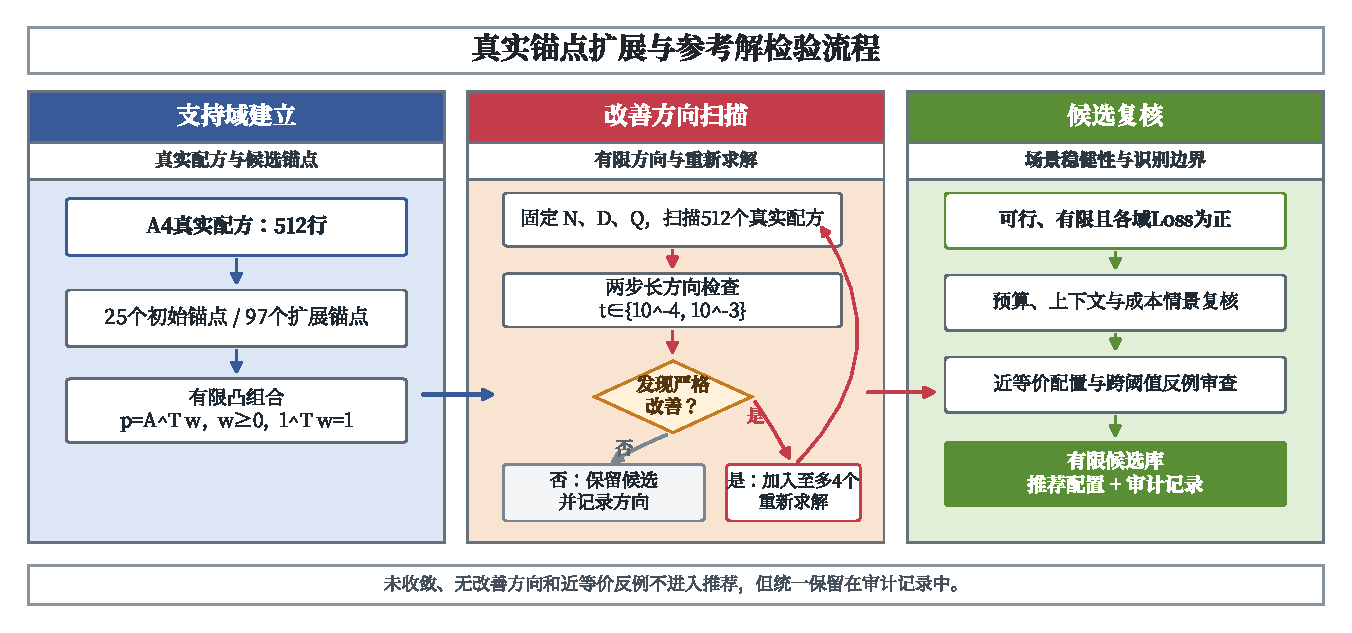
\includegraphics[width=.82\textwidth]{figures/flow_q3_model.pdf}
\caption{真实锚点扩展与参考解检验流程}
\label{fig:q3_4}
\end{figure}

\subsubsection{实验矩阵}

主实验覆盖 11 档预算、5 档上下文、3 种成本函数和 4 种决策方式。四种方式逐步释放 $N,D$、配比 $p$ 和治理质量 $Q$，用来分离规模、配比、治理和联合配置的贡献；成本归一化、桥接形式、收益强度、锚点集合、零收益和预算加密实验用于检验结论的稳定性。

\begin{table}[htbp]\centering\setlength{\tabcolsep}{3pt}\renewcommand{\arraystretch}{1.12}
\caption{四组消融与条件实验矩阵}\label{tab:q3_5}
\begin{tabularx}{\textwidth}{>{\raggedright\arraybackslash}p{2.975132cm}>{\raggedright\arraybackslash}p{7.933686cm}>{\raggedright\arraybackslash}X}\toprule
类别 & 自由变量或变化因素 & 数量及用途 \\
\midrule
规模基线 & $N,D$；固定平均配方与基础质量 & 联合配置的基准 \\
配比组 & $N,D,p$；固定基础质量 & 分离配比调整收益 \\
质量组 & $N,D,Q$；固定平均配方 & 分离治理收益及成本 \\
联合组 & $N,D,p,Q$ & 评价联合资源配置 \\
主矩阵 & 11预算、5上下文、3成本、4组 & 660项 \\
成本对照 & 统一 $Q_{\mathrm{base}}$ 至 1 的端点增量价格 & 检验价格尺度影响 \\
桥接对照 & 2种桥接、3种强度、2种基线质量 & 检验接口影响 \\
搜索敏感性 & 49/97锚点、6起点、边界扰动 & 检验求解稳定性 \\
零收益与预算加密 & $\kappa=0$；41档预算 & 检验治理收益与阈值 \\
算法对照 & 5预算、2上下文、3成本、2求解器 & 60项 \\
\bottomrule\end{tabularx}
\end{table}

\textbf{实验小结：} 求解层面由预算约束、正 Loss 检查、凸组合复核和多起点比较共同构成；实验层面由四组消融、五档上下文和三种成本函数共同回答“资源如何分配”和“结论是否依赖某一设定”两个问题。

\subsection{资源配置结果与结构性转移}

\subsubsection{联合收益与逐域代价}

以同预算、同上下文、同成本的规模基线为配对参照，定义平均改善率及非加性项

\begin{equation}\label{eq:q3_18}
G=100\frac{J_{\mathrm{base}}-J_{\mathrm{joint}}}{J_{\mathrm{base}}},\qquad
H=J_{\mathrm{quality}}+J_{\mathrm{mixture}}-J_{\mathrm{base}}-J_{\mathrm{joint}}.
\end{equation}

指数成本、上下文 4096 的四组轨迹见图~\ref{fig:q3_5}。165个原联合场景的平均改善率为 4.1603\%--5.8086\%，说明在本响应模型中同时释放配比和治理变量具有配置价值。$H$ 在 71 组为正、47 组为负、47 组接近零，联合收益随预算和响应曲率变化，并非固定的加法收益。

\begin{figure}[htbp]
\centering
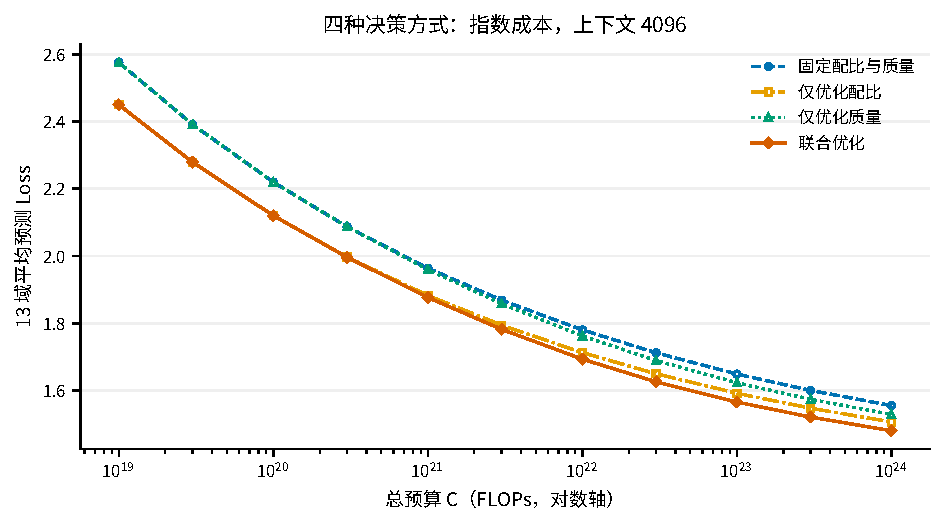
\includegraphics[width=.72\textwidth]{figures/result_q3_loss_ablation.pdf}
\caption{指数成本、上下文4096时11档预算的四组消融；各组均联动优化N/D}
\label{fig:q3_5}
\end{figure}

均值改善伴随领域间的重新分配。165组中有162组至少一个评测域的 Loss 上升，最多涉及2个领域；最大绝对退步为 0.0867182 nats，出现在 $C=3\times10^{20}$、上下文 2048、幂成本的 dm mathematics。图~\ref{fig:q3_6}展示三种成本和三档预算下的 13 域变化。

\begin{figure}[htbp]
\centering
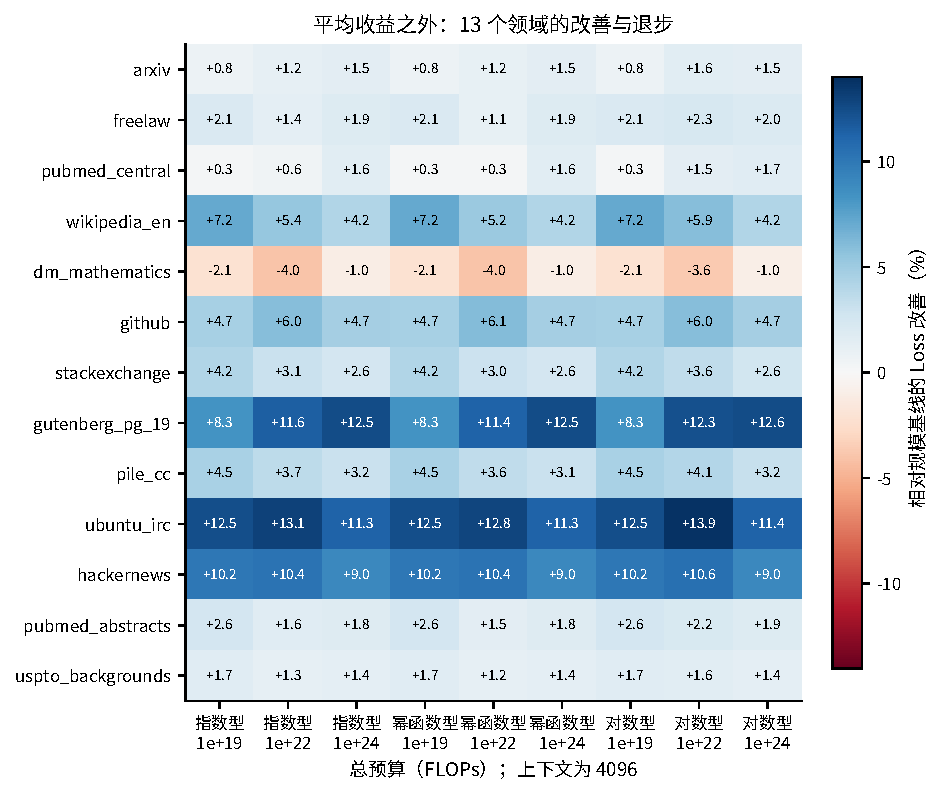
\includegraphics[width=.82\textwidth]{figures/result_q3_domain_tradeoffs.pdf}
\caption{典型配置的逐域代价；热力图保留13个评测域和9组预算--成本组合，颜色表示相对原配方的Loss变化}
\label{fig:q3_6}
\end{figure}

\FloatBarrier

\subsubsection{配方支持域与典型配置}

对全部 A4 配方作方向扫描后，165个原联合配置均发现 25 锚点域外的改善方向。上下文 4096 的33组扩域实验最终使用39--42个锚点，较原联合解进一步改善 0.8383\%--2.5512\%，配比 $L_1$ 变化为 0.5280--0.6468\%。图~\ref{fig:q3_7}呈现扩域收益，表~\ref{tab:q3_6}给出有限候选库中的典型配置。

\clearpage

\begin{figure}[t]
\centering
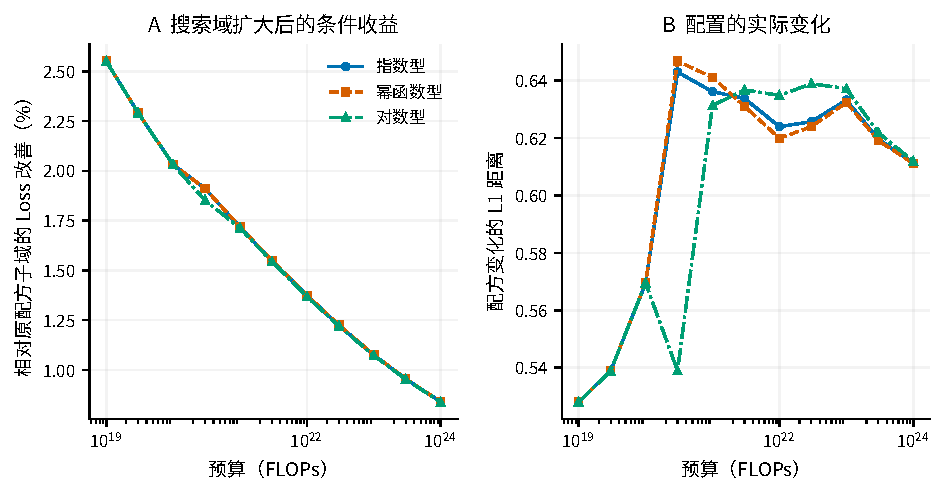
\includegraphics[width=.86\textwidth]{figures/result_q3_hull_expansion.pdf}
\caption{33个4096上下文配置的扩域结果相对原25锚点联合解的变化}\label{fig:q3_7}
\end{figure}

\begin{table}[htbp]\centering\setlength{\tabcolsep}{3pt}\renewcommand{\arraystretch}{1.12}
\caption{同合同有限候选库中的典型条件配置}\label{tab:q3_6}
\begin{tabularx}{\textwidth}{>{\raggedright\arraybackslash}p{2.487396cm}>{\raggedright\arraybackslash}p{1.989916cm}>{\raggedright\arraybackslash}p{2.288404cm}>{\raggedright\arraybackslash}p{2.387900cm}>{\raggedright\arraybackslash}p{1.691429cm}>{\raggedright\arraybackslash}p{2.089412cm}>{\raggedright\arraybackslash}X}\toprule
C（FLOPs） & 成本 & N（十亿） & D（十亿） & Q & J & 候选来源 \\
\midrule
$10^{19}$ & 指数 & 0.0678 & 21.64 & 0.6219 & 2.38753 & 扩展锚点 \\
$10^{19}$ & 幂 & 0.0678 & 21.64 & 0.6219 & 2.38753 & 扩展锚点 \\
$10^{19}$ & 对数 & 0.0678 & 21.64 & 0.6219 & 2.38753 & 扩展锚点 \\
$10^{22}$ & 指数 & 2.5115 & 491.40 & 0.9829 & 1.66994 & 扩展锚点 \\
$10^{22}$ & 幂 & 2.6199 & 452.13 & 1.0000 & 1.67192 & 扩展锚点 \\
$10^{22}$ & 对数 & 2.2175 & 626.41 & 1.0000 & 1.66062 & 97锚点 \\
$10^{24}$ & 指数 & 21.9273 & 6529.84 & 1.0000 & 1.46600 & 97锚点 \\
$10^{24}$ & 幂 & 22.0068 & 6480.02 & 1.0000 & 1.46612 & 97锚点 \\
$10^{24}$ & 对数 & 21.5744 & 6758.48 & 1.0000 & 1.46547 & 97锚点 \\
\bottomrule\end{tabularx}
\end{table}

幂成本、上下文 4096 下的三档典型配方见表~\ref{tab:q3_7}。低预算时三种成本均停留在 $Q_{\mathrm{base}}$；预算提高后，质量治理与配比调整开始共同占用新增算力。

\begin{table}[H]\centering\setlength{\tabcolsep}{3pt}\renewcommand{\arraystretch}{1.12}
\caption{幂成本条件下典型有限候选的完整领域配方（\%）}\label{tab:q3_7}
\begin{tabularx}{\textwidth}{>{\raggedright\arraybackslash}p{5.908112cm}>{\raggedright\arraybackslash}p{3.249462cm}>{\raggedright\arraybackslash}p{3.249462cm}>{\raggedright\arraybackslash}X}\toprule
领域 & $10^{19}$ & $10^{22}$ & $10^{24}$ \\
\midrule
arxiv & 3.45 & 2.62 & 1.79 \\
freelaw & 7.67 & 7.44 & 5.25 \\
nih exporter & 0.02 & 0.01 & 4.88 \\
pubmed central & 2.93 & 1.46 & 3.63 \\
wikipedia en & 6.84 & 7.74 & 19.69 \\
dm mathematics & 4.73 & 5.06 & 0.84 \\
github & 11.40 & 12.92 & 12.12 \\
philpapers & <0.005 & <0.005 & <0.005 \\
stackexchange & 14.07 & 13.10 & 3.83 \\
enron emails & 0 & <0.005 & 0.08 \\
gutenberg pg 19 & 6.55 & 9.03 & 15.90 \\
pile cc & 17.87 & 28.14 & 11.49 \\
ubuntu irc & 5.10 & 5.13 & 14.81 \\
europarl & <0.005 & <0.005 & 0.09 \\
hackernews & 6.16 & 4.63 & 5.22 \\
pubmed abstracts & 9.81 & 0.05 & <0.005 \\
uspto backgrounds & 3.41 & 2.67 & 0.36 \\
\bottomrule\end{tabularx}
\end{table}

\subsubsection{上下文、成本与结构状态}

图~\ref{fig:q3_8}表明，质量治理的绝对成本可随预算增加，而其在总成本中的份额未必增加。以扩域幂成本案例为例，预算从 $10^{22}$ 增至 $10^{24}$ 时，治理份额从 19.2241\% 降至 2.6935\%，治理绝对成本却从 $1.9224\times10^{21}$ 增至 $2.6935\times10^{22}$ FLOPs。图~\ref{fig:q3_9}给出规模与数据的局部资源平衡复核，165个原联合解的最大归一化残差为 $2.04434\times10^{-6}$。

\begin{figure}[htbp]
\centering
\begin{subfigure}[b]{.49\textwidth}
\centering
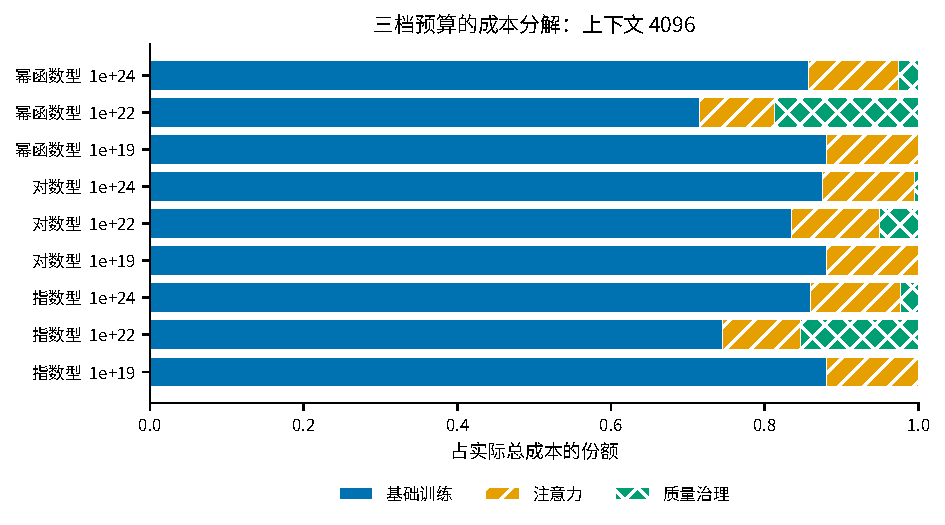
\includegraphics[width=.98\linewidth]{figures/result_q3_cost_allocation.pdf}
\caption{训练、注意力及治理份额}
\label{fig:q3_8}
\end{subfigure}\hfill
\begin{subfigure}[b]{.49\textwidth}
\centering
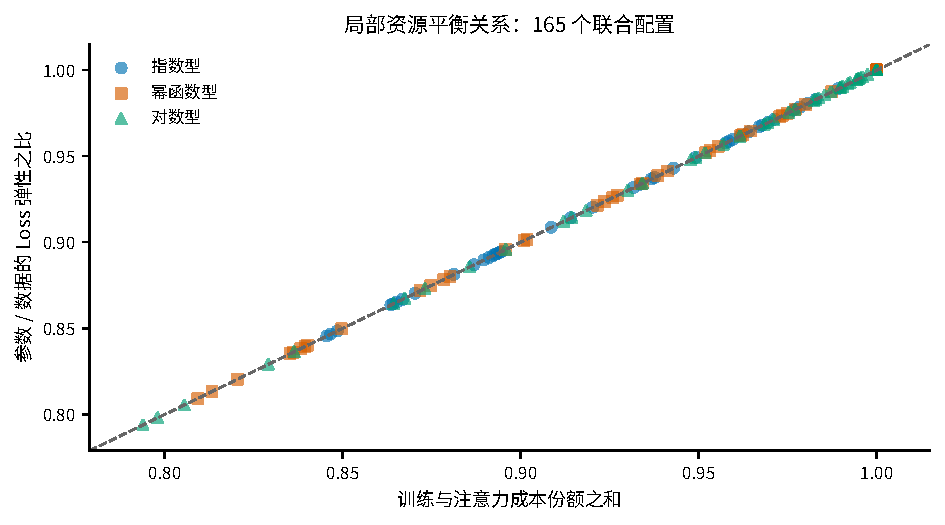
\includegraphics[width=.98\linewidth]{figures/process_q3_resource_balance.pdf}
\caption{资源均衡残差}
\label{fig:q3_9}
\end{subfigure}
\end{figure}

为区分价格尺度和函数形状，将三类成本在 $Q=1$ 处作端点归一化：

\begin{equation}\label{eq:q3_19}
\lambda_f=\frac{g_{\exp}(1)-g_{\exp}(Q_{\mathrm{base}})}{g_f(1)-g_f(Q_{\mathrm{base}})},
\qquad h_f^{\mathrm{norm}}(Q)=\lambda_f[g_f(Q)-g_f(Q_{\mathrm{base}})]_+.
\end{equation}

原价与归一化价格在55个预算--上下文组中有19组最优成本形式发生变化，说明成本曲线的价格量级和曲率都影响资源选择。相应轨迹见图~\ref{fig:q3_10}和图~\ref{fig:q3_11}。

\begin{figure}[htbp]
\centering
\begin{subfigure}[b]{.49\textwidth}
\centering
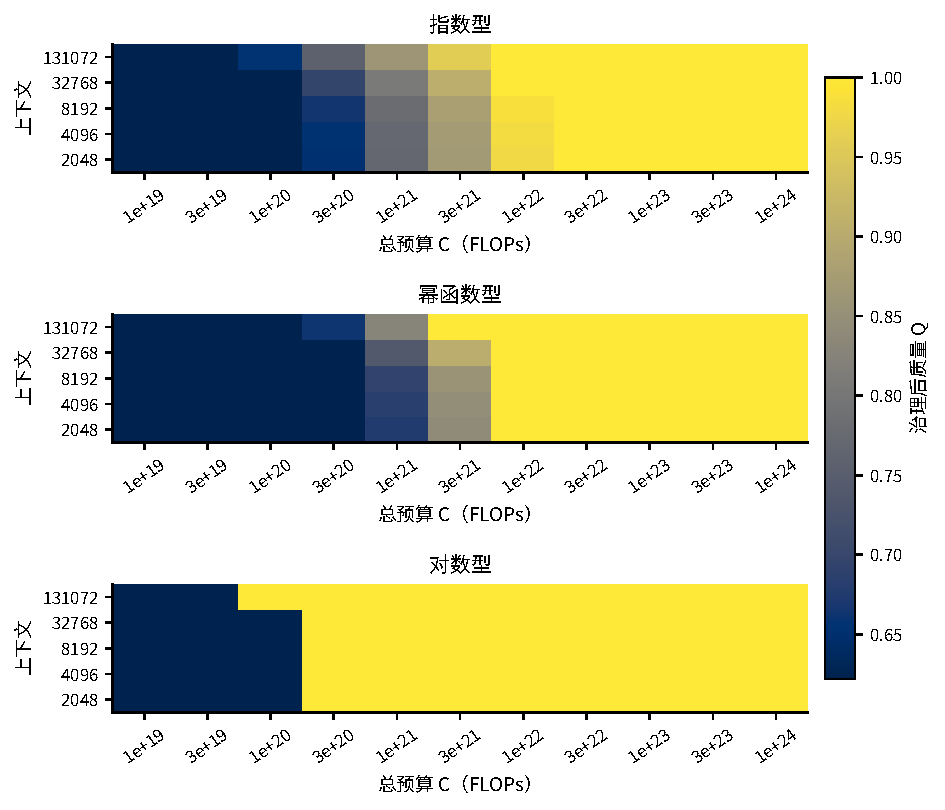
\includegraphics[width=.98\linewidth]{figures/result_q3_quality_regimes.pdf}
\caption{质量边界轨迹}
\label{fig:q3_10}
\end{subfigure}\hfill
\begin{subfigure}[b]{.49\textwidth}
\centering
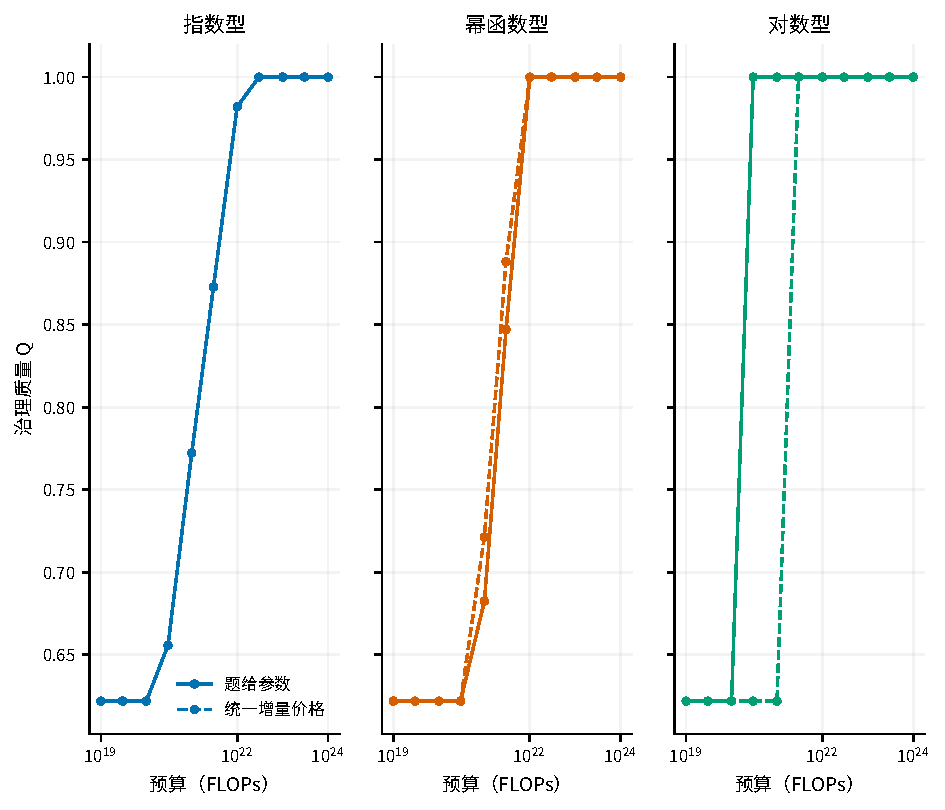
\includegraphics[width=.98\linewidth]{figures/result_q3_quality_cost_normalized.pdf}
\caption{归一化成本下的质量轨迹}
\label{fig:q3_11}
\end{subfigure}
\end{figure}

将结构性转移定义为最优状态的持续变化，而不是单个预算点的数值跳变。质量状态由 $Q$ 到质量上下界的距离确定；配方支持集与支持距离为

\begin{equation}\label{eq:q3_20}
S_\tau(p)=\{i:p_i>\tau\},\qquad
d_J(S_0,S_1)=1-\frac{|S_0\cap S_1|}{|S_0\cup S_1|},
\qquad \tau=0.01.
\end{equation}

配方变化同时满足 $d_J\ge0.2$ 与 $\|p_1-p_0\|_1\ge0.02$，并在后续预算点和加密预算中保持，才记为有效支持转移。机制方向、桥接形式、收益强度、随机种子、边界和锚点扰动共同构成情景检验；主支持比例门槛设为70\%。

\begin{table}[H]\centering\setlength{\tabcolsep}{3pt}\renewcommand{\arraystretch}{1.12}
\caption{结构转移识别与阈值敏感性}\label{tab:q3_8}
\begin{tabularx}{\textwidth}{>{\raggedright\arraybackslash}p{3.570159cm}>{\raggedright\arraybackslash}p{7.636173cm}>{\raggedright\arraybackslash}X}\toprule
项目 & 实际结果 & 判断 \\
\midrule
固定配方质量启动 & 指数成本、上下文131072出现一个下界至内点事件 & 质量治理由下界进入内点 \\
预算区间（FLOPs） & 粗：$[3\times10^{19},10^{20}]$；细：$[7.49894\times10^{19},10^{20}]$ & 两个区间属于同一事件 \\
情景支持比例 & 16/21，即76.19\% & 通过70\%门槛，未通过80\%门槛 \\
质量方向容差 & $10^{-4}$通过，$10^{-5}$不通过 & 阈值会影响事件识别 \\
联合配置 & 70\%门槛下没有稳定事件 & 联合策略未形成稳定结构转移 \\
光滑配方负对照 & 全部占比保持正值仍可跨1\%阈值 & 配方支持变化具有连续性 \\
\bottomrule\end{tabularx}
\end{table}

\textbf{结果小结：} 联合优化在平均 Loss 上取得 4.16\%--5.81\% 的改善，但改善由领域间让渡伴随而来；扩展 A4 支持域后，配置仍可进一步改善。上下文变长持续挤压 $N$ 和 $D$，成本函数的价格尺度与曲率都会改变治理轨迹。结构检验在固定配方、指数成本、最长上下文条件下发现一个质量启动事件；在联合配置的多情景检验中，没有形成稳定的结构转移。

\subsection{稳健性检验与问题三结论}

\subsubsection{有限情景的稳健配置}

对同一组候选在两种桥接和三种正收益强度下进行六情景复算。设 $X$ 为共同可行候选集，定义

\begin{equation}\label{eq:q3_21}
J_s^{\mathrm{best}}=\min_{x\in X}J_s(x),\qquad
R_s(x)=\frac{J_s(x)-J_s^{\mathrm{best}}}{|J_s^{\mathrm{best}}|}.
\end{equation}

以最小化最大后悔值选择稳健候选：

\begin{equation}\label{eq:q3_22}
x_{\mathrm{rob}}\in\mathop{\arg\min}_{x\in X}\max_sR_s(x),\qquad
v_{\mathrm{rob}}=\min_{x\in X}\max_sR_s(x).
\end{equation}

165组的最大相对后悔值为1.5465\%，零收益压力情景下为2.5946\%。这说明推荐配置对已登记桥接和收益强度具有有限幅度的稳定性；稳健性结论随候选库和情景集合一并定义。

\begin{figure}[htbp]
\centering
\begin{subfigure}[b]{.49\textwidth}
\centering
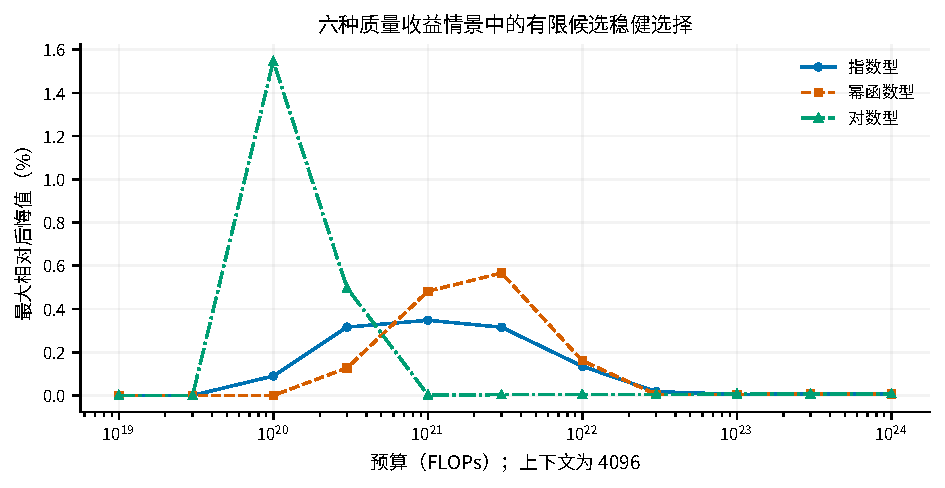
\includegraphics[width=.98\linewidth]{figures/result_q3_finite_regret.pdf}
\caption{有限候选的情景后悔值}
\label{fig:q3_12}
\end{subfigure}\hfill
\begin{subfigure}[b]{.49\textwidth}
\centering
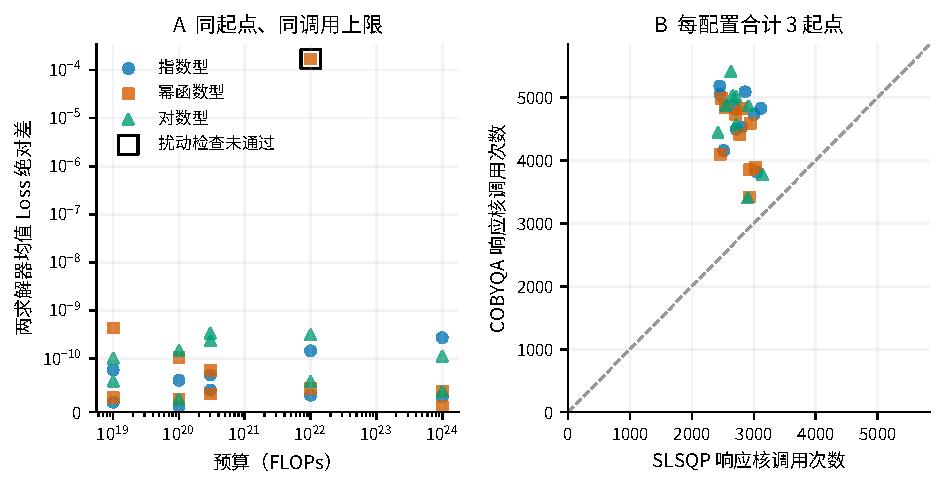
\includegraphics[width=.98\linewidth]{figures/process_q3_solver_agreement.pdf}
\caption{两种求解器的一致性}
\label{fig:q3_13}
\end{subfigure}
\end{figure}

\subsubsection{求解器复算与适用范围}

SLSQP 与 COBYQA 在相同 25 锚点、相同 3 起点和相同配置上进行 30 对复算。60个结果均满足基本可行条件，扰动检查通过 59 个；SLSQP 为 30/30，COBYQA 为 29/30，最大均值 Loss 差为 0.000168474。求解器复算、有限后悔和零收益对照共同表明，推荐结果不是某一个局部搜索设置的单点产物。

本问计算的是第二问响应函数下的条件配置，质量桥接沿用 B7 标尺，配方支持来自 A4，实际上下文来自 C7。后续实证步骤是：先以表~\ref{tab:q3_6}选择预算和上下文下的候选，再在同一数据治理流水线上记录真实治理 FLOPs，并用 13 域评测 Loss 对 $Q$、$g(Q)$ 和桥接强度重新校准。

\textbf{问题三结论：}
\begin{enumerate}
    \item 在总成本 $C=D[(6+\eta_{\mathrm{attn}}L_{\mathrm{ctx}})N+h(Q)]$ 下，联合优化变量为 $N,D,Q,w$，配比由 $p=A^{\mathsf T}w$ 生成；这同时满足算力预算、质量上下界、尺度范围和真实配方支持约束。
    \item 在当前响应模型中，联合释放配比和治理质量使平均 Loss 改善 4.1603\%--5.8086\%，但 165 组中 162 组至少有一个评测域退步，实际部署应根据领域优先级增加逐域约束。
    \item 上下文长度通过注意力成本直接改变可用于 $N$ 和 $D$ 的预算；$L_{\mathrm{ctx}}^{\mathrm{crit}}=30000$，C7 中的 32768 和 131072 已进入注意力成本高于训练成本的区间。成本函数的价格尺度和曲率都会改变治理质量轨迹。
    \item 结构检验在固定配方、指数成本、上下文131072下发现一次质量由下界进入内点的事件；联合配置未形成通过70\%情景门槛的稳定结构转移。有限候选最大相对后悔值为1.5465\%，求解器复算的合格率为59/60。
\end{enumerate}
